\documentclass[11pt,a4paper]{article}
\usepackage{isabelle,isabellesym}
\usepackage{graphicx}
\graphicspath {{figures/}}

% further packages required for unusual symbols (see also
% isabellesym.sty), use only when needed


\usepackage{latexsym}
\usepackage{amssymb}
  %for \<leadsto>, \<box>, \<diamond>, \<sqsupset>, \<mho>, \<Join>,
  %\<lhd>, \<lesssim>, \<greatersim>, \<lessapprox>, \<greaterapprox>,
  %\<triangleq>, \<yen>, \<lozenge>

%\usepackage[greek,english]{babel}
  %option greek for \<euro>
  %option english (default language) for \<guillemotleft>, \<guillemotright>

%\usepackage[latin1]{inputenc}
  %for \<onesuperior>, \<onequarter>, \<twosuperior>, \<onehalf>,
  %\<threesuperior>, \<threequarters>, \<degree>

%\usepackage[only,bigsqcap]{stmaryrd}
  %for \<Sqinter>

%\usepackage{eufrak}
  %for \<AA> ... \<ZZ>, \<aa> ... \<zz> (also included in amssymb)

%\usepackage{textcomp}
  %for \<cent>, \<currency>

% this should be the last package used
\usepackage{pdfsetup}

% urls in roman style, theory text in math-similar italics
\urlstyle{rm}
\isabellestyle{it}

\begin{document}

% sane default for proof documents
\parindent 0pt\parskip 0.5ex

\title{Belief Revision Theory}
\author{ Valentin Fouillard \and Safouan TAHA \and Frederic Boulanger \and Nicolas Sabouret}
\maketitle

\newpage

\begin{abstract}
The 1985 paper by Carlos Alchourrón, Peter Gärdenfors,
and David Makinson (AGM), “On the Logic of Theory Change: Partial Meet Contraction and Revision Functions” launches a large and rapidly growing literature that employs formal models and logics to handle changing beliefs of a rational agent and to take into account new piece of information observed by this agent. In 2011, a review book titled "AGM 25 Years: Twenty-Five Years of Research in Belief Change" was edited to summarize the first twenty five years of works based on AGM.

This  HOL-based  AFP entry is a faithful formalization of the AGM operators (e.g. contraction, revision, remainder ...) axiomatized in the original paper. It also contains the proofs of all the theorems stated in the paper that show how these operators combine. Both proofs of Harper and Levi identities are established.
\end{abstract}

\newpage

\tableofcontents

\newpage

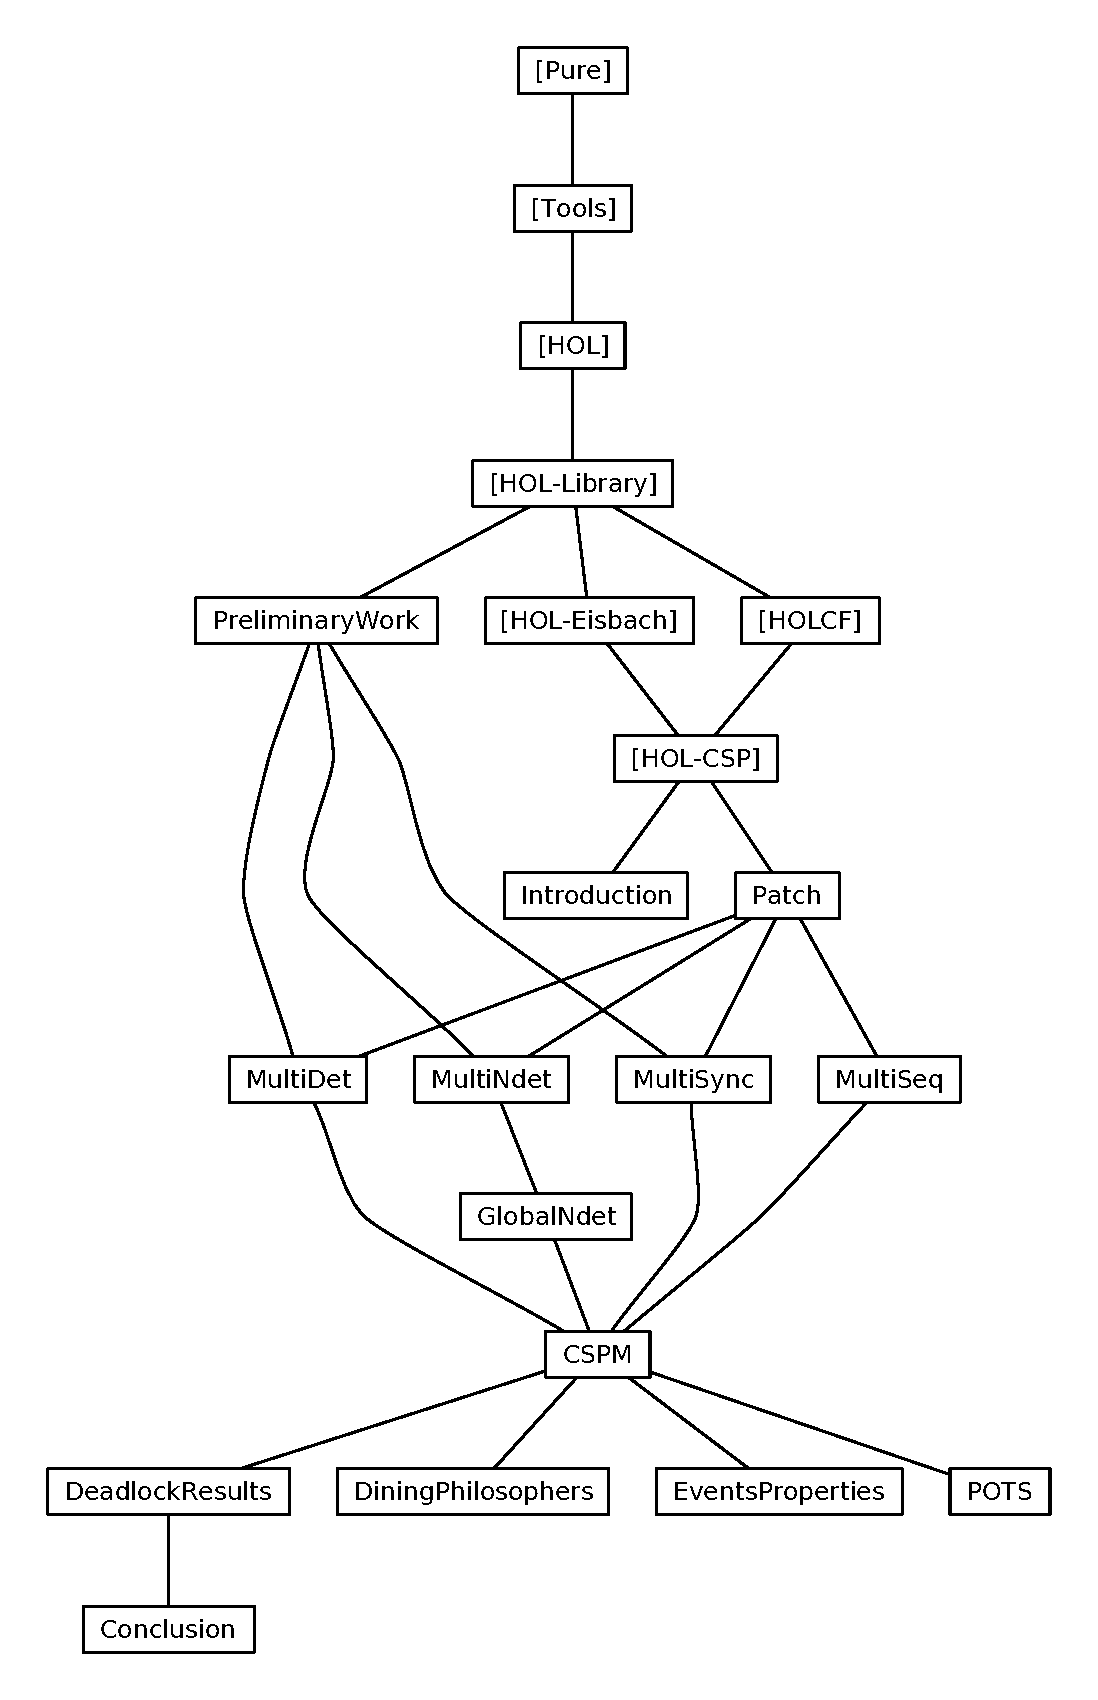
\includegraphics{session_graph.pdf}

\newpage

% generated text of all theories
\input{session}

% optional bibliography
\bibliographystyle{abbrv}
\bibliography{adb-long,root}

\end{document}


%%% Local Variables:
%%% mode: latex
%%% TeX-master: t
%%% End:
